\documentclass[12pt,a4paper]{article}
\usepackage[hagavi]{azzam}
\usepackage{tikz}
\usepackage{float}
\usepackage{graphicx}

\title{Soal Geometri OSK SMA 2016--2026 (No.\ 11--20)}
\author{Compiled by Azzam}
\date{\today}

\begin{document}
\maketitle

\begin{enumerate}

% osk sma 2016 nomor 11 (bagian 11--20)
% Geometri: G3. Teorema Pythagoras dan Perbandingan Trigonometri
\item (OSK SMA 2016 No.\ 11) Segitiga $ABC$ mempunyai panjang sisi $AB=20$, $AC=21$, dan $BC=29$. Titik $D$ dan $E$ terletak pada segmen garis $BC$, dengan $BD=8$ dan $EC=9$. Besar $\angle DAE$ adalah \dots derajat.

% osk sma 2016 nomor 15 (bagian 11--20)
% Geometri: G2. Luas dan Keliling Bangun Gabungan
\item (OSK SMA 2016 No.\ 15) Diberikan persegi $ABCD$ dengan panjang sisi 1. Titik $K$ dan $L$ berturut-turut terletak pada segmen garis $BC$ dan $DC$ sehingga keliling dari $\triangle KCL$ adalah 2. Luas minimum dari $\triangle AKL$ adalah \dots

% osk sma 2016 nomor 19 (bagian 11--20)
% Geometri: G12. Segiempat Konsiklis
\item (OSK SMA 2016 No.\ 19) Diberikan empat titik pada satu lingkaran $\Gamma$ dalam urutan $A, B, C, D$. Sinar garis $AB$ dan $DC$ berpotongan di $E$, dan sinar garis $AD$ dan $BC$ berpotongan di $F$. Misalkan $EP$ dan $FQ$ menyinggung lingkaran $\Gamma$ berturut-turut di $P$ dan $Q$. Misalkan pula bahwa $EP=60$ dan $FQ=63$, maka panjang $EF$ adalah \dots

% osk sma 2017 nomor 12 (bagian 11--20)
% Geometri: G4. Garis-Garis Istimewa Segitiga
\item (OSK SMA 2017 No.\ 12) Diberikan segitiga $ABC$ dengan $AC=\frac{1}{2}(AB+BC)$. Misalkan $K$ dan $M$ berturut-turut titik tengah $AB$ dan $BC$. Titik $L$ terletak pada sisi $AC$ sehingga $BL$ adalah garis bagi sudut $ABC$. Jika $\angle ABC=72^{\circ}$, maka besarnya sudut $KLM$ sama dengan \dots

% osk sma 2017 nomor 16 (bagian 11--20)
% Geometri: G3. Teorema Pythagoras dan Perbandingan Trigonometri
\item (OSK SMA 2017 No.\ 16) Pada segitiga $ABC$ titik $K$ dan $L$ berturut-turut adalah titik tengah $AB$ dan $AC$. Jika $CK$ dan $BL$ saling tegak lurus, maka nilai minimum dari $\cot B + \cot C$ adalah \dots

% osk sma 2017 nomor 17 (bagian 11--20)
% Geometri: G7. Geometri Analitik
\item (OSK SMA 2017 No.\ 17) Misalkan $a, b, c,$ dan $d$ bilangan-bilangan bulat positif. Jajargenjang yang dibatasi oleh garis-garis $y=ax+c$, $y=ax+d$, $y=bx+c$, dan $y=bx+d$ mempunyai luas 18. Jajargenjang yang dibatasi oleh garis-garis $y=ax+c$, $y=ax-d$, $y=bx+c$, dan $y=bx-d$ mempunyai luas 72. Nilai terkecil yang mungkin untuk $a+b+c+d$ adalah \dots

% osk sma 2017 nomor 20 (bagian 11--20)
% Geometri: G4. Garis-Garis Istimewa Segitiga
\item (OSK SMA 2017 No.\ 20) Diberikan segitiga $ABC$ dengan $AB=12$, $BC=5$ dan $AC=13$. Misalkan $P$ suatu titik pada garis bagi $\angle A$ yang terletak di dalam $ABC$ dan misalkan $M$ suatu titik pada sisi $AB$ (dengan $A\ne M\ne B$). Garis $AP$ dan $MP$ memotong $BC$ dan $AC$ berturut-turut di $D$ dan $N$. Jika $\angle MPB = \angle PCN$ dan $\angle NPC = \angle MBP$, maka nilai $\frac{AP}{PD}$ adalah \dots

% osk sma 2018 nomor 13 (bagian 11--20)
% Geometri: G2. Luas dan Keliling Bangun Gabungan
\item (OSK SMA 2018 No.\ 13) Misalkan $ABCD$ adalah trapesium siku-siku dengan $AB$ sejajar $DC$ dan $AB$ tegak lurus $AD$. Misalkan juga $P$ adalah titik potong diagonal $AC$ dan $BD$. Jika perbandingan luas segitiga $APD$ dan luas trapesium $ABCD$ adalah $4:25$ maka nilai $\frac{AB}{DC}$ adalah \dots

% osk sma 2018 nomor 16 (bagian 11--20)
% Geometri: G12. Segiempat Konsiklis
\item (OSK SMA 2018 No.\ 16) Diberikan segitiga $ABC$ dan lingkaran $\Gamma$ yang berdiameter $AB$. Lingkaran $\Gamma$ memotong sisi $AC$ dan $BC$ berturut-turut di titik $D$ dan $E$. Jika $AD=\frac{1}{3}AC$, $BE=\frac{1}{4}BC$ dan $AB=30$ maka luas segitiga $ABC$ adalah \dots

% osk sma 2018 nomor 20 (bagian 11--20)
% Geometri: G12. Segiempat Konsiklis
\item (OSK SMA 2018 No.\ 20) Pada segitiga $ABC$, panjang sisi $BC$ adalah 1 satuan. Ada tepat satu titik $D$ pada sisi $BC$ yang memenuhi $|DA|^{2}=|DB|\cdot|DC|$. Jika $k$ menyatakan keliling $ABC$, jumlah semua nilai $k$ yang mungkin adalah \dots

% osk sma 2019 nomor 12 (bagian 11--20)
% Geometri: G9. Transformasi Geometri
\item (OSK SMA 2019 No.\ 12) Diberikan segitiga $ABC$ dengan $D$ pertengahan $AC$, $E$ pertengahan $BD$, dan $H$ merupakan pencerminan dari $A$ terhadap $E$. Jika $F$ perpotongan antara $AH$ dengan $BC$, maka nilai $\frac{AF}{FH}$ sama dengan \dots

% osk sma 2019 nomor 15 (bagian 11--20)
% Geometri: G5. Lingkaran
\item (OSK SMA 2019 No.\ 15) Misalkan $ABCD$ adalah persegi dengan panjang sisi 4. Lingkaran-lingkaran $x, y, z$ dengan jari-jari sama mempunyai pusat di dalam persegi sedemikian sehingga lingkaran $x$ menyinggung sisi $AB$ dan $AD$, lingkaran $y$ menyinggung sisi $AB$ dan $BC$, serta lingkaran $z$ menyinggung sisi $DC$, lingkaran $x$, dan lingkaran $y$. Diketahui jari-jari lingkaran $x$ dapat dinyatakan dengan $n-\sqrt{m}$ dengan $m$ dan $n$ bilangan bulat positif. Nilai $m$ adalah \dots

% osk sma 2019 nomor 17 (bagian 11--20)
% Geometri: G6. Segiempat dan Poligon
\item (OSK SMA 2019 No.\ 17) Diberikan jajar genjang $ABCD$, dengan $\angle ABC=105^{\circ}$. Titik $M$ berada di dalam jajar genjang sehingga segitiga $BMC$ sama sisi dan $\angle CMD=135^{\circ}$. Jika $K$ pertengahan sisi $AB$, maka besarnya $\angle BKC$ sama dengan \dots derajat.

% osk sma 2020 nomor 11 (bagian 11--20)
% Geometri: G12. Segiempat Konsiklis
\item (OSK SMA 2020 No.\ 11) Diberikan segitiga $ABC$ dengan $\angle ACB=48^{\circ}$. Garis bagi $\angle BAC$ memotong sisi $BC$ dan lingkaran luar $ABC$ berturut-turut di titik $D$ dan $E$. Jika $AC=AB+DE$, maka $\angle ABC=\dots$

% osk sma 2020 nomor 15 (bagian 11--20)
% Geometri: G2. Luas dan Keliling Bangun Gabungan
\item (OSK SMA 2020 No.\ 15) Misalkan $ABC$ segitiga dan $P, Q, R$ titik pada sisi $BC, CA, AB$. Jika luas segitiga $ABC$ sama dengan 20 kali luas segitiga $PQR$ dan $\frac{AQ}{AC}+\frac{BR}{BA}+\frac{CP}{CB}=1$, maka $\left(\frac{AQ}{AC}\right)^{2}+\left(\frac{BR}{BA}\right)^{2}+\left(\frac{CP}{CB}\right)^{2}=\dots$

% osk sma 2020 nomor 20 (bagian 11--20)
% Geometri: G4. Garis-Garis Istimewa Segitiga
\item (OSK SMA 2020 No.\ 20) Misalkan $H$ adalah titik tinggi dari segitiga lancip $ABC$ dan $P$ adalah titik tengah $CH$. Jika $AP=3$, $BP=2$ dan $CP=1$, maka panjang sisi $AB$ adalah \dots (Catatan: Titik tinggi suatu segitiga adalah perpotongan ketiga garis tinggi dari segitiga tersebut.)

% osk sma 2021 nomor 15 (bagian 11--20)
% Geometri: G5. Lingkaran
\item (OSK SMA 2021 No.\ 15) Diberikan segitiga $ABC$ dengan $AB=6$, $BC=7$, dan $CA=8$. Jika $I$ adalah titik potong ketiga garis bagi segitiga $ABC$, maka $AI^{2}$ adalah \dots

\begin{figure}[H]
    \centering
    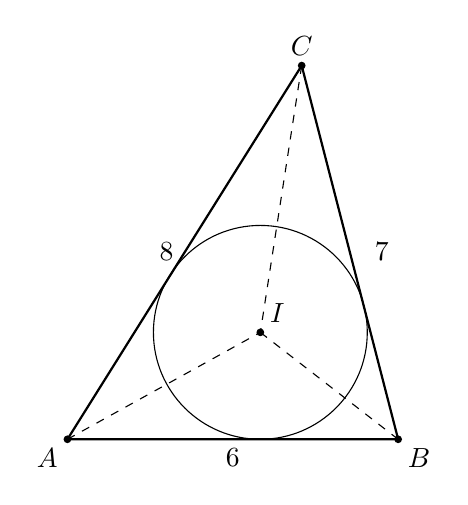
\begin{tikzpicture}[scale=0.7]
        \coordinate (A) at (0,0);
        \coordinate (B) at (6,0);
        \coordinate (C) at (4.25,6.78);
        \coordinate (I) at (3.5,1.94);
        \draw[thick] (A) -- (B) -- (C) -- cycle;
        \draw[dashed] (A) -- (I);
        \draw[dashed] (B) -- (I);
        \draw[dashed] (C) -- (I);
        \draw[thin] (I) circle (1.94);
        \fill (A) circle (2pt) node[below left] {$A$};
        \fill (B) circle (2pt) node[below right] {$B$};
        \fill (C) circle (2pt) node[above] {$C$};
        \fill (I) circle (2pt) node[above right] {$I$};
        \node[below] at (3,0) {$6$};
        \node[right] at (5.4,3.4) {$7$};
        \node[left] at (2.1,3.4) {$8$};
    \end{tikzpicture}
\end{figure}

% osk sma 2021 nomor 20 (bagian 11--20)
% Geometri: G5. Lingkaran
\item (OSK SMA 2021 No.\ 20) Diberikan segitiga siku-siku $ABC$ dengan $\angle C=90^{\circ}$. Titik $D$ terletak pada sisi $AB$ dan $E$ terletak pada sisi $AC$ sehingga $DE$ sejajar dengan garis $BC$. Diketahui setengah lingkaran berwarna biru, merah, hijau sedemikian sehingga setengah lingkaran biru menyinggung $AC$ dan $AB$, setengah lingkaran merah menyinggung sisi $AB$ dan garis $DE$, dan setengah lingkaran hijau menyinggung setengah lingkaran biru dan $DE$. Jika $2AC+5BC=5AB$, maka perbandingan jari-jari setengah lingkaran merah dan setengah lingkaran hijau adalah $k : 25$. Nilai $k$ adalah \dots

\begin{figure}[H]
    \centering
    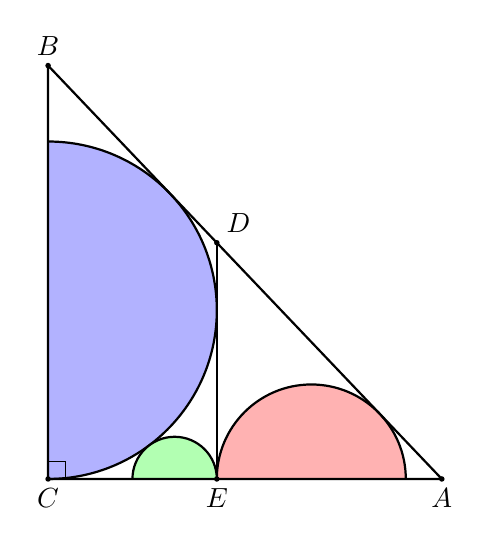
\begin{tikzpicture}[scale=0.25]
        % BC : AC : AB = 21 : 20 : 29 from 2AC + 5BC = 5AB
        \coordinate (C) at (0,0);
        \coordinate (A) at (20,0);
        \coordinate (B) at (0,21);
        \coordinate (E) at ({60/7},0);
        \coordinate (D) at ({60/7},12);
        \fill[blue!30] (0,0) arc (-90:90:{60/7}) -- cycle;
        \draw[thick] (0,0) arc (-90:90:{60/7});
        \fill[red!30] ({60/7},0) arc (180:0:4.8) -- cycle;
        \draw[thick] ({60/7},0) arc (180:0:4.8);
        \fill[green!30] ({30/7},0) arc (180:0:{15/7}) -- cycle;
        \draw[thick] ({30/7},0) arc (180:0:{15/7});
        \draw[thick] (A) -- (B) -- (C) -- cycle;
        \draw[thick] (E) -- (D);
        \draw (0.9,0) -- (0.9,0.9) -- (0,0.9);
        \fill (A) circle (4pt) node[below] {$A$};
        \fill (B) circle (4pt) node[above] {$B$};
        \fill (C) circle (4pt) node[below] {$C$};
        \fill (D) circle (4pt) node[above right] {$D$};
        \fill (E) circle (4pt) node[below] {$E$};
    \end{tikzpicture}
\end{figure}

% osk sma 2022 nomor 12 (bagian 11--20)
% Geometri: G5. Lingkaran
\item (OSK SMA 2022 No.\ 12) Diberikan segitiga siku-siku $ABC$. Jika luas dari segitiga $ABC$ adalah 112. Misalkan $R$ adalah panjang jari-jari lingkaran luar segitiga $ABC$ dan $r$ adalah panjang jari-jari lingkaran dalam segitiga $ABC$. Diketahui juga $R+r=16$. Panjang sisi miring dari segitiga $ABC$ adalah \dots

% osk sma 2022 nomor 15 (bagian 11--20)
% Geometri: G4. Garis-Garis Istimewa Segitiga
\item (OSK SMA 2022 No.\ 15) Diberikan $ABC$ siku-siku sama kaki dengan panjang $BC=AB$ dan $L$ titik tengah $BC$. Titik $P$ pada sisi $AC$ sehingga $BP$ tegak lurus dengan $AL$. Jika panjang $CP=30\sqrt{2}$, panjang $AB$ adalah \dots

% osk sma 2022 nomor 19 (bagian 11--20)
% Geometri: G6. Segiempat dan Poligon
\item (OSK SMA 2022 No.\ 19) Diberikan belah ketupat $ABCD$ dan titik $E$ ada di dalam $ABCD$ sehingga panjang $AE=BE$. Jika $\angle BAE=12^{\circ}$ dan $\angle DAE=72^{\circ}$, besar $\angle CDE$ dalam satuan derajat adalah \dots

% osk sma 2023 nomor 11 (bagian 11--20)
% Geometri: G12. Segiempat Konsiklis
\item (OSK SMA 2023 No.\ 11) Diberikan segiempat $ABCD$ siklis dengan lingkaran luarnya adalah $\omega$. Panjang $BC = CD$, $AC$ memotong $BD$ di titik $E$, $BE=7$, dan $DE=4$. Garis singgung $\omega$ di titik $A$ memotong $BD$ di titik $P$. Jika $\frac{PD}{PB}$ dapat ditulis dalam bentuk $\frac{m}{n}$ dengan $m$ dan $n$ adalah bilangan asli yang saling relatif prima, nilai dari $m+n$ adalah \dots

% osk sma 2023 nomor 15 (bagian 11--20)
% Geometri: G5. Lingkaran
\item (OSK SMA 2023 No.\ 15) Diberikan lingkaran $\Omega$ dan $AB$ merupakan tali busur dari $\Omega$.

\begin{center}
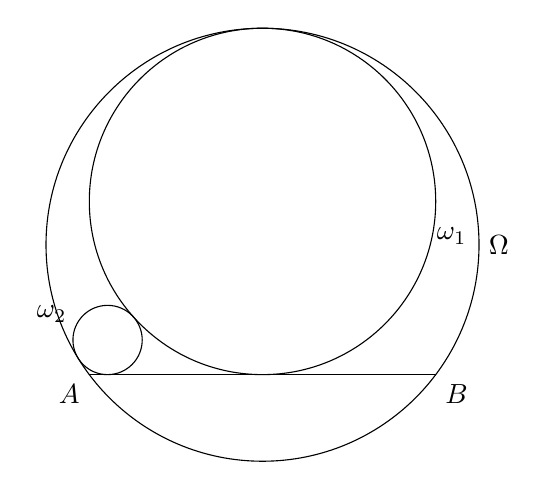
\begin{tikzpicture}[scale=0.055]
    \draw (0,30) circle (50);
    \draw (0,40) circle (40);
    \draw (-35.78,8) circle (8);
    \draw (-40,0) -- (40,0);
    \node[below left] at (-40,0) {$A$};
    \node[below right] at (40,0) {$B$};
    \node[right] at (50,30) {$\Omega$};
    \node[right] at (38,32) {$\omega_{1}$};
    \node[left] at (-43,14) {$\omega_{2}$};
\end{tikzpicture}
\end{center}

Lingkaran $\omega_{1}$ menyinggung $\Omega$ secara internal dan menyinggung $AB$ pada titik tengahnya. Lingkaran $\omega_{2}$ menyinggung $\Omega$ secara internal, dan $\omega_{1}$ secara eksternal serta menyinggung $AB$. Jika jari-jari dari $\omega_{1}$ adalah 40 dan jari-jari dari $\omega_{2}$ adalah 8, panjang dari $AB$ adalah \dots

% osk sma 2023 nomor 19 (bagian 11--20)
% Geometri: G4. Garis-Garis Istimewa Segitiga
\item (OSK SMA 2023 No.\ 19) Diberikan segitiga $ABC$. Misal titik $D, E, F$ terletak pada sisi $BC, CA, AB$ sehingga $AD, BE, CF$ berpotongan di satu titik. Diketahui bahwa $\angle EDF=56^{\circ}$. Jika $\angle ADB=90^{\circ}$ dan $AF=FB$, maka besar $\angle ABC$ adalah \dots

% osk sma 2024 nomor 11 (bagian 11--20)
% Geometri: G2. Luas dan Keliling Bangun Gabungan
\item (OSK SMA 2024 No.\ 11) Suatu segienam beraturan disisipkan ke dalam sebuah persegi panjang seperti terlihat pada gambar di bawah ini. Jika luas $A$ dan $B$ berturut-turut adalah 24 dan 28, maka luas segienam beraturan adalah \dots

\begin{center}
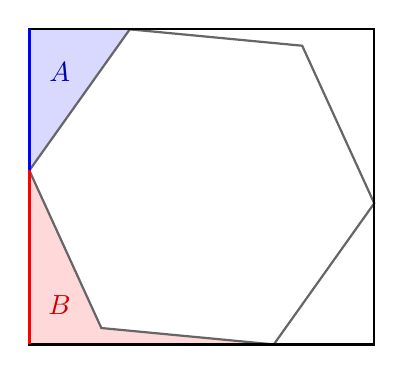
\begin{tikzpicture}[scale=1.1]
    \fill[blue!15] (0,3.6379) -- (1.1595,3.6379) -- (0,2.0083) -- cycle;
    \fill[red!15] (0,0) -- (2.8225,0) -- (0.8315,0.1894) -- (0,2.0083) -- cycle;
    \draw[thick,black!60] (0,2.0083) -- (1.1595,3.6379) -- (3.1505,3.4485) -- (3.9820,1.6296) -- (2.8225,0) -- (0.8315,0.1894) -- cycle;
    \draw[thick] (0,0) rectangle (3.9820,3.6379);
    \draw[very thick,blue] (0,3.6379) -- (0,2.0083);
    \draw[very thick,red] (0,2.0083) -- (0,0);
    \node[blue!70!black] at (0.35,3.15) {$A$};
    \node[red!80!black] at (0.35,0.45) {$B$};
\end{tikzpicture}
\end{center}

% osk sma 2024 nomor 16 (bagian 11--20)
% Geometri: G5. Lingkaran
\item (OSK SMA 2024 No.\ 16) Diberikan sebuah segitiga $ABC$ yang siku-siku pada sudut $B$. Lingkaran $\omega$ merupakan lingkaran dalam segitiga $ABC$ yang menyinggung sisi $BC$ pada titik $D$. Titik $E$ terletak pada $\omega$ sehingga $DE$ merupakan diameter $\omega$. Perpanjangan garis $AE$ memotong $\omega$ kedua kalinya di titik $F$ dan memotong sisi $BC$ di titik $G$. Apabila $EF=3$ dan $FG=4$ maka panjang $AE$ dapat dinyatakan dalam bentuk $\frac{p}{r}\sqrt{q}$ dengan $p,q,r$ merupakan bilangan bulat positif, satu-satunya faktor kuadrat dari $q$ adalah 1, dan $\text{FPB}(p,r)=1$. Nilai dari $p+q+r$ adalah \dots

% osk sma 2024 nomor 20 (bagian 11--20)
% Geometri: G12. Segiempat Konsiklis
\item (OSK SMA 2024 No.\ 20) Pada segitiga $ABC$, titik $D$ dan $E$ terletak pada garis $BC$ sehingga $B, D, E, C$ terletak pada urutan tersebut. Diketahui bahwa $BD:DE:EC=4:2:5$ dan garis-garis $AD, AE$ membagi tiga $\angle BAC$ sama besar. Garis $AD$ dan $AE$ masing-masing memotong lingkaran luar $ABC$ pada titik $F$ dan $G$. Nilai dari $\frac{DF}{EG}$ dapat dinyatakan dalam bentuk $\sqrt{\frac{p}{q}}$ untuk suatu bilangan bulat positif $p$ dan $q$ yang relatif prima, nilai dari $p+q$ adalah \dots

% osk sma 2025 nomor 12 (bagian 11--20)
% Geometri: G12. Segiempat Konsiklis
\item (OSK SMA 2025 No.\ 12) Diketahui sebuah lingkaran pusat titik $O$ dan jari-jari 65. Titik $A, B, C$ merupakan tiga titik berbeda pada lingkaran tersebut dan titik $D, E, F$ berturut-turut merupakan titik tengah $BC, CA, AB$. Jika dua ruas garis $OD, OE, OF$ memiliki panjang 25 dan 39, maka panjang ruas garis yang ketiga adalah \dots

% osk sma 2025 nomor 16 (bagian 11--20)
% Geometri: G9. Transformasi Geometri
\item (OSK SMA 2025 No.\ 16) Diketahui persegi panjang $ABCD$ dan $E$ suatu titik pada sisi $AB$. Suatu benda bergerak dari titik $A$ dan berturut-turut menyentuh sisi $BC, CD, AD$ dan sampai titik $E$. Berikut diberikan sebuah contoh lintasan dari benda tersebut.

\begin{center}
\begin{tikzpicture}[scale=0.7]
    \coordinate (A) at (0,0);
    \coordinate (B) at (0,6);
    \coordinate (C) at (8.5,6);
    \coordinate (D) at (8.5,0);
    \coordinate (E) at (0,5);
    \coordinate (T) at (7.4,6);
    \coordinate (R) at (8.5,4.7);
    \coordinate (S) at (4.5,0);
    \draw (A) -- (B) -- (C) -- (D) -- cycle;
    \draw[densely dashed] (A) -- (T) -- (R) -- (S) -- (E);
    \fill (A) circle (2.5pt);
    \fill (B) circle (2.5pt);
    \fill (C) circle (2.5pt);
    \fill (D) circle (2.5pt);
    \fill (E) circle (2.5pt);
    \fill (T) circle (2pt);
    \fill (R) circle (2pt);
    \fill (S) circle (2pt);
    \node[below] at (A) {A};
    \node[above left] at (B) {B};
    \node[above right] at (C) {C};
    \node[below] at (D) {D};
    \node[left] at (E) {E};
\end{tikzpicture}
\end{center}

Jika diketahui $AB=60$, $AD=85$, dan jarak terpendek yang ditempuh oleh benda tersebut adalah $170\sqrt{2}$, maka panjang $AE$ adalah \dots

% osk sma 2026 nomor 14 (bagian 11--20)
% Geometri: G1. Garis, Sudut, dan Segitiga
\item (OSK SMA 2026 No.\ 14) Terdapat sebuah segitiga sama sisi $ABC$. Titik $M$ dan $N$ terletak di $BC$ dan $M\ne N$. Titik $D$ terletak di dalam segitiga $ABC$ sehingga $DMN$ segitiga sama sisi. Garis $BD$ memotong garis $AC$ di $E$ dan garis $CD$ memotong garis $AB$ di $F$. Jika $MN=3$, $BF=4$, dan $CE=8$, panjang $BC$ adalah \dots

% osk sma 2026 nomor 16 (bagian 11--20)
% Geometri: G5. Lingkaran
\item (OSK SMA 2026 No.\ 16) Terdapat dua lingkaran dengan titik pusat $O_{1}$ dan $O_{2}$ dengan jari-jari 4 dan 8. Dua lingkaran tersebut berpotongan di $X$ dan $Y$ dengan $\angle O_{1}XO_{2}=90^{\circ}$. Dibuat garis singgung persekutuan luar yang lebih dekat ke $X$ daripada $Y$, menyinggung lingkaran $O_{1}$ di $A$ dan $O_{2}$ di $B$. Misalkan garis $AB$ memotong garis $XY$ di $P$. Luas dari segitiga $O_{1}PO_{2}$ adalah \dots

% osk sma 2026 nomor 17 (bagian 11--20)
% Geometri: G2. Luas dan Keliling Bangun Gabungan
\item (OSK SMA 2026 No.\ 17) Diberikan segitiga $ABC$. Titik $D$ pada $AB$ sehingga $\frac{AD}{DB}=\frac{7}{4}$ dan titik $E$ pada $AC$ sehingga $\frac{AE}{EC}=\frac{3}{8}$. Misalkan $M$ adalah titik tengah $BC$ dan $N$ adalah titik potong $AM$ dan $DE$. Jika luas dari segitiga $ABC$ adalah 1210, luas dari segitiga $ADN$ adalah \dots

\end{enumerate}

\end{document}